\section{The Aharonov-Bohm Effect, Scattering Intro}
\subsection{Review of the Argument - Vector Potentials are Physical in QM}
Again, we want to explore the deep question of Gauge invariance in quantum mechanics. It is important to understand how to do it incorrectly. We discussed the scenario where we had a solenoid of width $a$, and with a charged particle $q$ on a ring $R$ around the solenoid. We have the Hamiltonian:
\begin{equation}
    H = \frac{1}{2m}\left(\v{p} - \frac{e}{c}\v{A}\right)^2
\end{equation}
note that outside the solenoid, the field is zero $\v{B} = \v{0}$ but the Gauge potential is nonzero $\v{A} \neq 0$. Under a Gauge transformation:
\begin{equation}
    \v{A}' = \v{A} + \nabla \Lambda
\end{equation}
which induces the transformation on the wavefunction $\psi' = e^{i\frac{e}{\hbar c}\Lambda(\v{r})}\psi$.

There were two ways of solving this we could say there is always way of bringing $\v{A}' = \v{0}$ under a Gauge transformation (and we could say we don't care about the phase factor); then we get the simple result:
\begin{equation}
    E_l = \frac{\hbar^2}{2mR^2}l^2
\end{equation}

This solution is \emph{WRONG}!! If we solve the problem correctly with the Gauge potential, we find that the spectrum is actually different:
\begin{equation}
    E_l = \frac{\hbar^2}{2mR^2}\left(l - \frac{e\Phi}{2\pi\hbar c}\right)^2
\end{equation}
(though so long as the flux is quantized, we recover the same result). But the conclusion is extremely, extremely nontrivial. Even though there is no field at the location of the particle, the particle knows that the solenoid is there! In QM not only is the $\v{B}$-field physical, but so is the vector potential $\v{A}$. 

\subsection{Quantization of Flux}

We can explicitly write $\Lambda(\v{r})$ as the following:
\begin{equation}
    \Lambda(\v{r}) = \int_{0, \Gamma}^r \v{A} \cdot d\v{l}
\end{equation}
where we integrate over the path. What went wrong with our first solution? We see that:
\begin{equation}
    e^{i\frac{e}{\hbar c}\Lambda(\v{r})} = e^{i\frac{e}{\hbar c}\int_{0, \Gamma}^r \v{A} \cdot d\v{l}}
\end{equation}

If we take a complete cycle, the integral above is nothing but the flux:
\begin{equation}
    \oint \v{A} \cdot d\v{l} = \int \v{B} \cdot d\v{a} = \Phi
\end{equation}
If the flux is quantized, we are not sensitive to it:
\begin{equation}
    \frac{e}{\hbar c}\Phi = 2\pi n
\end{equation}
as we then have $e^{2\pi i n} = 1$ and the phase vanishes. This is a famous formula in CM physics (if we take $e \to 2e$ for type-II superconductivity).

One takeaway is we can make gauge transformation if the wavefunction is single valued. Otherwise, we cannot.

\subsection{The Aharonov-Bohm Effect}
Recall the two-slit experiment. If we don't observe the electrons as they go through the slits, then we get a diffraction pattern. If we do observe the electron as they go through the slits, this breaks the diffraction pattern and we have two peaks at the same place as the slits.

We consider now placing a solenoid behind the two slits (as pictured below) such that the $\v{B}$-field never touches the electrons. Does this have an effect on the interference pattern? Indeed, it does. Let us try to understand why this is the case. 

\begin{figure}[htbp]
    \centering
    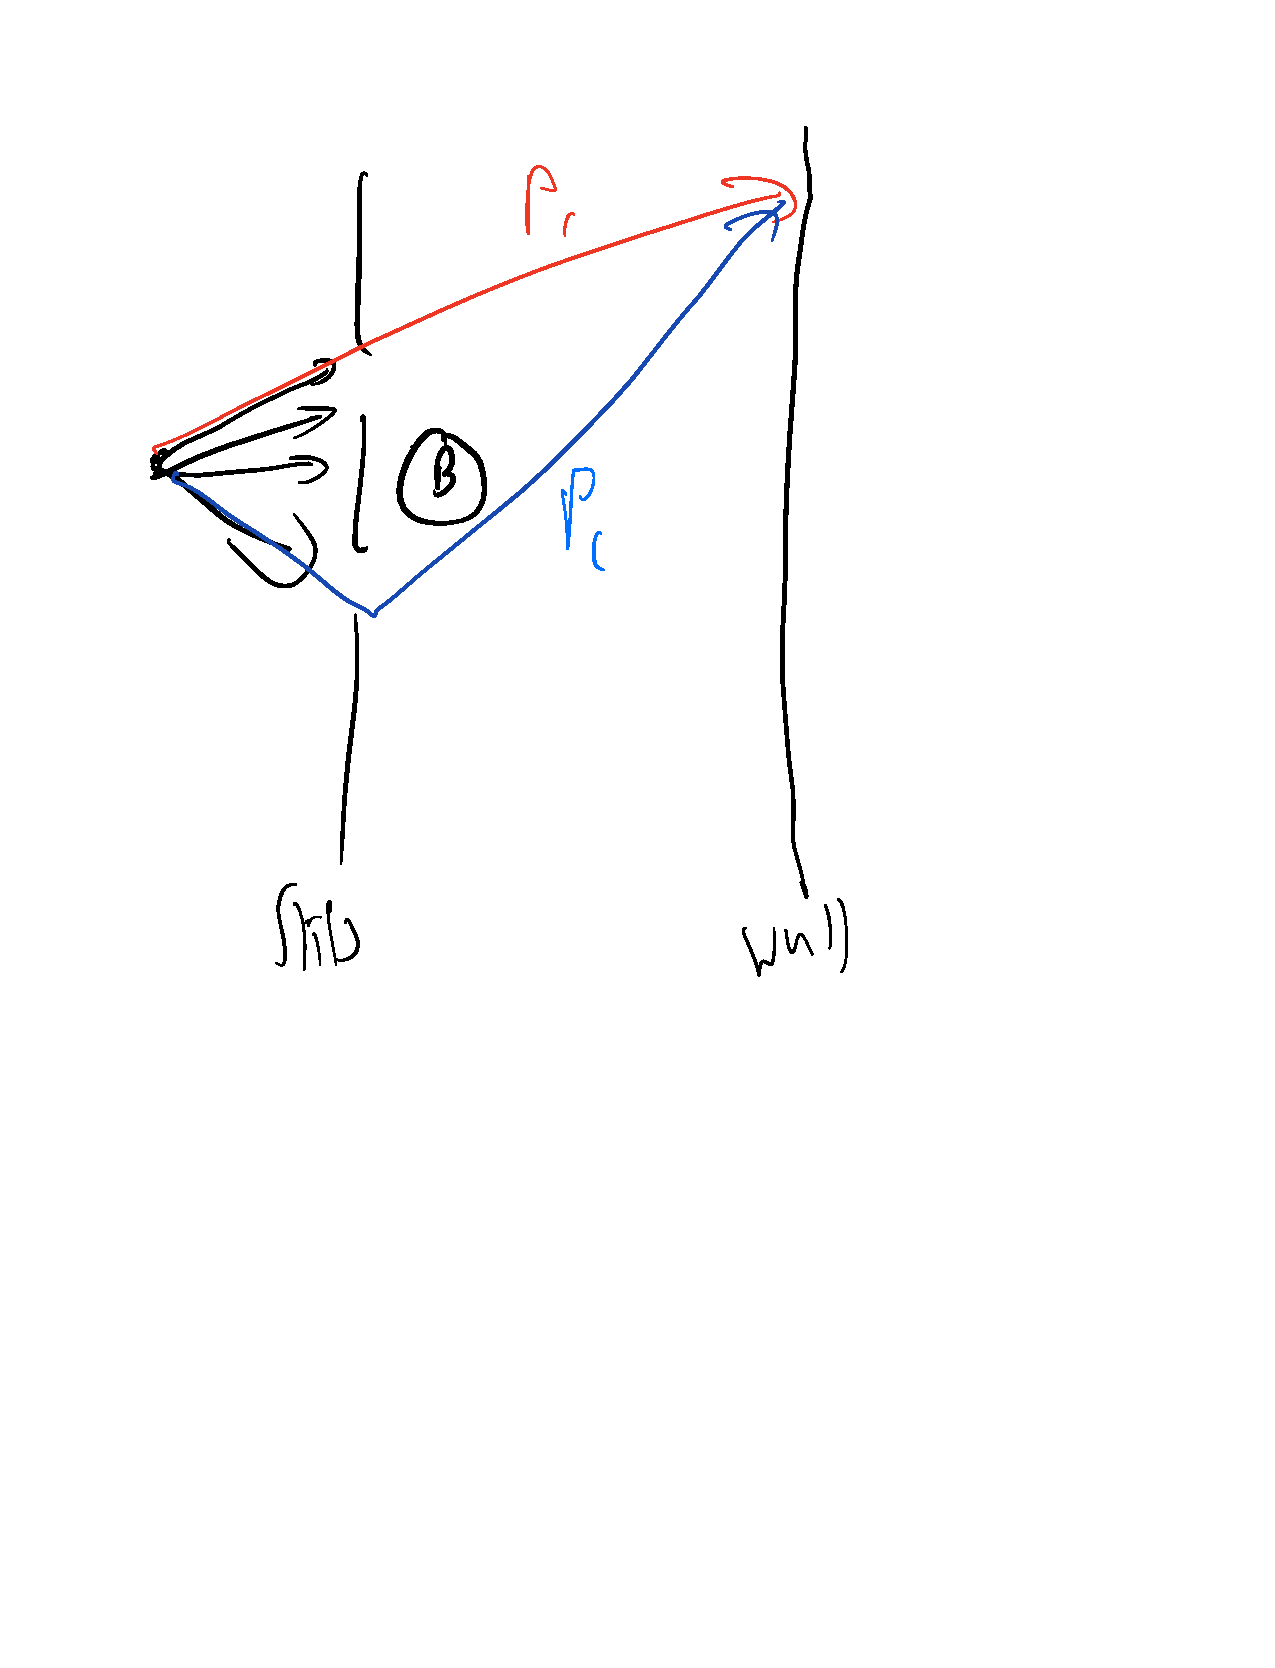
\includegraphics[scale=0.5]{Images/fig-ABeffect.pdf}
    \caption{Sketch of the A-B effect setup.}
    \label{fig-ABeffect}
\end{figure}

Our wavefunction along the first path is:
\begin{equation}
    \psi_1 = \psi_0 e^{i\frac{e}{\hbar c}\int_{r_0, \Gamma_1}^{r_1}\v{A} \cdot d\v{r}}
\end{equation}
and along the second path:
\begin{equation}
    \psi_2 = \psi_0 e^{i\frac{e}{\hbar c}\int_{r_0, \Gamma_2}^{r_1} \v{A} \cdot d\v{r}}
\end{equation}
What is the intensity at $r_1$? We can superimpose the wavefunctions:
\begin{equation}
    \psi_1 + \psi_2 = e^{i\frac{e}{\hbar c}\int_{r_0, \Gamma_1}^r \v{A} \cdot d\v{r}}\left[\psi_0 + \psi_0e^{i\frac{e}{\hbar c}\int_{r_0, \Gamma_2}^r}e^{-i\frac{e}{\hbar c}\int_{r_0, \Gamma_1}^r \v{A} \cdot d\v{r}}\right]
\end{equation}
The second term we can write as a path integral around the closed loop:
\begin{equation}
    \psi_0 e^{i\frac{e}{\hbar c}\oint_{\Gamma = \Gamma_1 + \Gamma_2}\v{A} \cdot d\v{r}} = \psi_0 e^{i\frac{e}{\hbar c}\Phi}
\end{equation}
where the loop integral just gives the magnetic flux! Our superposition is therefore:
\begin{equation}
    \psi_1 + \psi_2 = \psi_0\left[1 + e^{i\frac{e}{\hbar c}\Phi}\right]
\end{equation}
where we have neglected the global phase. Note that we have avoided the very hard computation of the path integral over $\v{A}$ by using Stoke's theorem, rewriting this integral (in the case of a closed loop) as the total flux. This is a very interesting result! this is a topological phenomena (essentially - the difference ) - if the solenoid is outside the loop, we see no effect, and if the solenoid if inside the loop, we do an effect!

Note - $\v{A}$ is not \emph{physical} in a literal sense, but the loop integral over it is, and it does impact physics! See holonomy in math if you want the technical discussion\dots

Also note - this is a simple manifestation of the much more general Berry's phase.

A final comment about magnetic monopoles. In classical electromagnetism, $\nabla \cdot \v{B} = \v{0}$ and there is no magnetic monopoles. This can also be experimentally verified. Nevertheless, we search for them (and Gordon Semenoff is part of a collaboration to search for them!)! It goes back to an old story by Dirac, who says they do not exist in classical E\&M but you find them in quantum. Dirac suggests that you have a magnetic field, and then there is a string attached with a quantized flux $\frac{e}{\hbar c}\Phi = 2\pi n$. If I touch the string, I can resolve the Maxwell equations. The total flux is zero because of the magnetic monpole inside and the string outside, but it is integer and therefore not observable. This is a way that magnetic charge is quantized - this is the famous Dirac quantization argument for magnetic monpoles. CM physicists discuss magnetic monopoles all the time as well - however note these are monopoles in momentum-space.

\subsection{Intro to Scattering - Elastic scattering}
We start with an intuitive picture and then develop the theory precisely. Fermi's golden rule tells us that:
\begin{equation}
    \dod{W}{t} = \frac{2\pi}{\hbar}\abs{V_{fi}}^2 \delta[E_f - E_i]\frac{Vd^3p}{(2\pi\hbar)^3}
\end{equation}
As we discussed in WKB, we compute the phase volume and get the number of quantum cells etc.

Now, we apply this to scattering. We have some initial state:
\begin{equation}
    \ket{\psi_i} \cong e^{i\frac{\v{p}_i \cdot \v{r}}{\hbar}}\frac{1}{\sqrt{V}}e^{-i\frac{E_i t}{\hbar}}
\end{equation}
The final state is:
\begin{equation}
    \bra{\psi_f} \cong e^{-i\frac{\v{p}_f \cdot \v{r}}{\hbar}}\frac{1}{\sqrt{V}}e^{i\frac{E_f t}{\hbar}}
\end{equation}
Note when we take the inner product we get the term:
\begin{equation}
    e^{i\frac{E_f - E_i}{\hbar}t} = e^{i\omega t}
\end{equation}
Fermi's Golden rule comes from this time-dependent part. The $\abs{V_{if}}^2$ is the $\v{r}$ dependent part - 
\begin{equation}
    \bra{\psi_f}V\ket{\psi_i} = \int d^3r e^{-i\frac{\v{p}_f \cdot \v{r}}{\hbar}}e^{i\frac{\v{p}_i \cdot \v{r}}{\hbar}} V_{int}(\v{r})
\end{equation}
with $V_{int}$ the interaction potential. We therefore have the matrix elements:
\begin{equation}
    V_{fi} = \int d^3r e^{-i\v{q} \cdot \v{r}}V_{int}(\v{r})
\end{equation}
where $\v{q} = \frac{\v{p}_f - \v{p}_i}{\hbar}$ s the momentum transfer. $V_{fi}$ we note to be the Fourier transform of the original potential! Let us integrate over all momentum of the final states, then:
\begin{equation}
    \dod{W}{t} = \frac{2\pi}{\hbar}\frac{d^3p_f}{(2\pi\hbar)^3}\frac{V}{V^2}\abs{\tilde{U}(\v{q})}^2\delta(E_f - E_i)
\end{equation}
Where $\tilde{U} = \int V(r)e^{-i\v{q} \cdot \v{r}}$. We can actually do the integration here, as the delta function is easily evaluated (we've already done it):
\begin{equation}
    \int d^3p_f \delta(E_f - E_i) = \int p_f^2 dp_f d\Omega_f\delta(\frac{p_f^2}{2m} - \frac{p_i^2}{2m})
\end{equation}
We assume elastic scattering here, so $p_f = p_i$ We can carry out this integral by considering:
\begin{equation}
    int d^3p_f \delta(E_f - E_i) = \int \frac{p_f}{2}dp_f^2 \delta(\frac{p_f^2}{2m} - \frac{p_i^2}{2m})d\Omega = \int \frac{2m\abs{p_i}}{2}d\Omega_f = \int \frac{2m\abs{p_f}}{2}d\Omega_f
\end{equation}
so then:
\begin{equation}
    \dod{W}{t} = \frac{2\pi}{\hbar}\frac{1}{(2\pi\hbar)}^3\frac{m\abs{p_f}d\Omega_f}{V}\abs{\tilde{U}(\v{q})}^2
\end{equation}
note that we have not done the normalization yet to make this a cross-section. We will consider this next day.